\newpage
\section{Beschreibung der Module}
	\subsection{Kurbeschreibung}
	Das gesamte Projekt besteht auf folgenden Modulen (Flussdiagramme sind im Kapitel~\ref{Module}):
	\begin{description}[font=\sffamily\bfseries, leftmargin=1.5cm,style=sameline] 
	\item{\textbf{main}}
	Dies ist das Hauptprogramm. Beim Start werden die serielle Schnittstelle und das \textbf{scheduler}-Modul initialisiert. Das Konsolenprozess wird erzeugt. Timer-Interrupts werden initialisiert. Danach befindet sich das Hauptprogramm in einer Endlosschleife.
	
	\item{\textbf{proc\_console}}
	Dies ist der Konsolenprozess. Der Prozess ist eine Endlosschleife, welche die Eingaben von der seriellen Schnittstelle abholt. Diese Eingaben werden auf �bereinstimmung mit den bekannten Befehlen gepr�ft. Unbekannte Eingaben werden verworfen. Befehle werden erkannt und ausgef�hrt.
	\item{\textbf{scheduler}} Dies ist der eigentliche Task-Verwalter. Das Modul besteht aus Subroutinen:
	\begin{description}[font=\sffamily\bfseries, leftmargin=0.5cm,style=sameline] 
	\item{\textbf{new\_proc}}
		Hier wird ein neuer Prozess erzeugt. In der Prozesstabelle im externen RAM wird nach dem ersten freien Platz gesucht (first fit). Jeder Prozess wird vereinfacht gleich gro� angenommen.
		Die Position des gefundenen freien Platzes in der Prozesstabelle entspricht einer Position vom Datenbereich der Prozesse. Die Datenbereiche werden initialisiert.
		
	\item{\textbf{del\_proc}} Hier wird der Verweis auf den Datenbereich eines zu beendenden Prozesses aus der Prozesstabelle entfernt. Hiermit kennt der Task-Verwalter diesen Prozess und seinen Datenbereich nicht mehr.
	
	\item{\textbf{change\_proc}}
	Hier wird der Kontext der Prozesse getauscht. Hierbei werden alle prozessrelevanten Daten in den externen Speicher ausgelagert (�hnlich wie Swapping). N�chster Prozess wird aus der Prozesstabelle geholt und sein Kontext wird ins RAM geladen.
	
	\end{description} 
	
	\item{\textbf{serial}} Dieses Modul stellt Routinen zum I/O auf der seriellen Schnittstelle bereit.
	
	\item{\textbf{proc\_a}} Prozess a: Eine Zeichenfolge \textquotedblleft abcde\textquotedblright wird auf der seriellen Schnittstelle 0 ausgegeben.
	\item{\textbf{proc\_b}} Prozess b: Gibt jede Sekunde \textquotedblleft+\textquotedblright auf die serielle Schnittstelle aus
	\item{\textbf{proc\_z}} Prozess z: Ruft fkt\_text auf
	\item{\textbf{fkt\_text}} Testprozess: gibt eine Zeichenfolge auf serielle Schnittstelle 1 aus.
	\end{description}
	
\newpage
\subsection{Speichernutzung und Variablen}

F�r das Programm werden folgende Speicherbereiche reserviert und verwendet:

\subsubsection*{Variablen und Konstanten}

Variablen und Konstanten werden im \textquotedblleft variables.inc\textquotedblright{} dem Befehl \begin{center}
<NAME> EQU <HEX>
\end{center} angelegt. Durch einbinden der Datei in jedes Modul sind die Variablen global bekannt. Die genaue Beschreibung der Variablen und deren Funktion ist einem  kommentierten Listing im Anhang zu entnehmen.

\subsubsection{Externer Datenbereich}
Externer Datenbereich wird folgenderma�en genutzt. Zu Beginn des Programms werden zwei Datenbereiche im externen Speicher reserviert. Ein Bereich ist die Prozesstabelle. Pro Prozess sind hier 4 Byte vergeben. Die setzen sich wie folgt zusammen. 2 Byte DPTR auf den dazugeh�rigen Prozessdatenbereich, 1 Byte Bitmaske mit Prozessstatus und Prozesstyp und 1 Byte f�r die Prozess ID.

Es sind insgesamt 20 Prozesse m�glich. Die Entscheidung f�r die Zahl 20 ist willk�rlich und kann auch generell auf \textquotedblleft beliebig\textquotedblright{} gesetzt werden. Die Grenze bildet hier die Gr��e des externen Datenbereichs. 

Jeder Prozess besitzt seinen eigenen Datenbereich, worin sein Kontext aufbewahrt wird. Pro Prozess sind 32 Byte reserviert. Aktuell werden lediglich 23 Byte benutzt. 10 Byte f�r den Stack und 13 Byte f�r den geforderten Kontext. Eine Erweiterung der Stackgr��e ist m�glich. Abbildung~\ref{fig:ext_data} zeigt die Speicherbelegung. 
\begin{figure}[H]
\centering
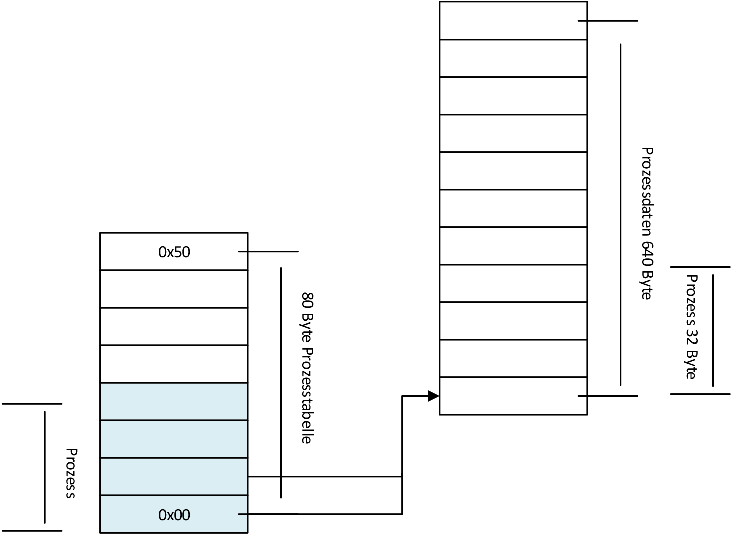
\includegraphics[width=0.7\textwidth]{./images/ext_data}
\caption{Speicherbelegung des externen RAM}
\label{fig:ext_data}
\end{figure}

Die Abbildung~\ref{fig:dataprocess} zeigt die reale Speicherbelegung eines eingelagerten Prozesses. Dabei sind die kleineren Adressen unten.

\begin{figure}[H]
\centering
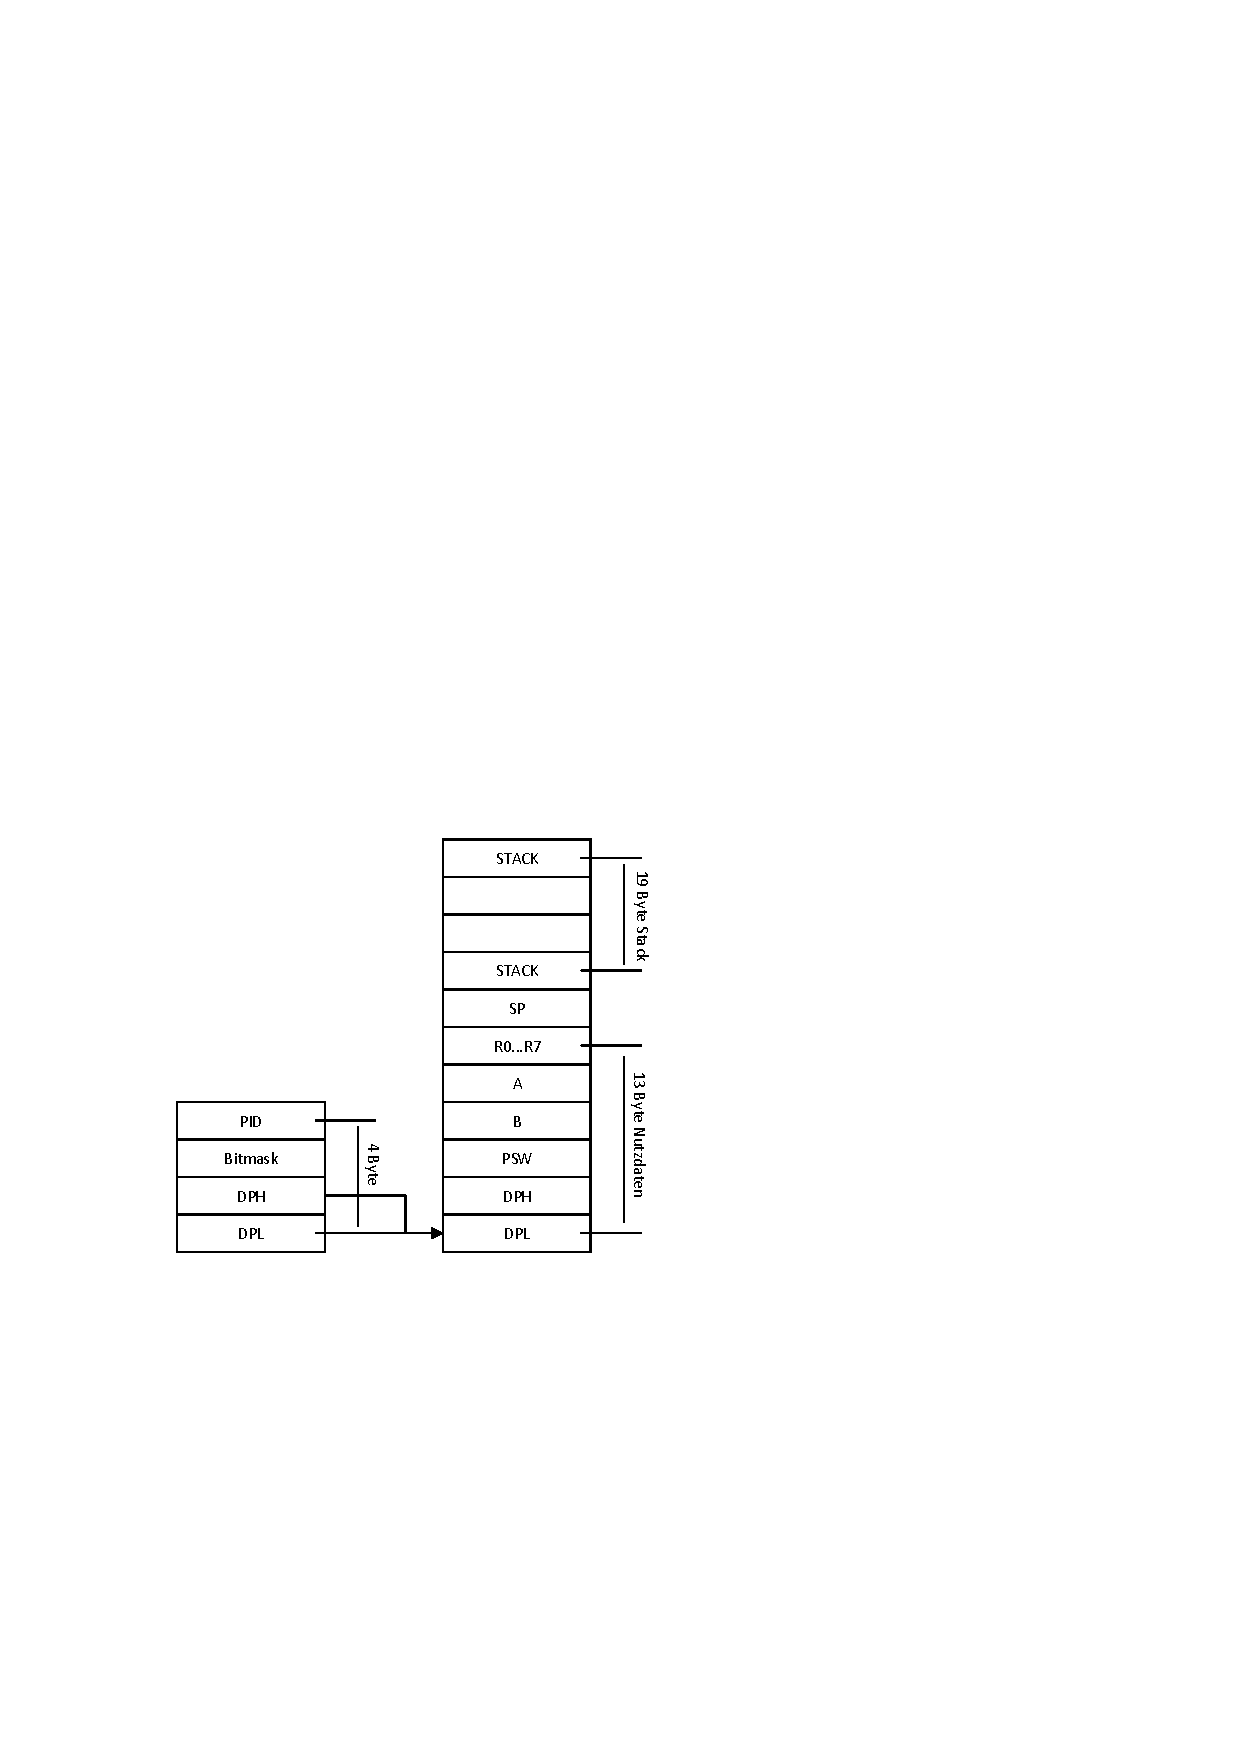
\includegraphics[width=0.7\textwidth]{./images/data_process}
\caption{Speicherbelegung des externen RAM f�r einen Prozess}
\label{fig:dataprocess}
\end{figure}
\newpage
\subsection{Module\label{Module}}
\subsubsection{Hauptmodul \texttt{main.a51}}
In der Abbildung~\ref{fig:main} ist das Ablaufdiagramm vom Hauptmodul dargestellt. Die genaue Beschreibung der einzelnen Operationen ist aus dem Listing im Anhang zu entnehmen.

\begin{figure}[H]
\centering
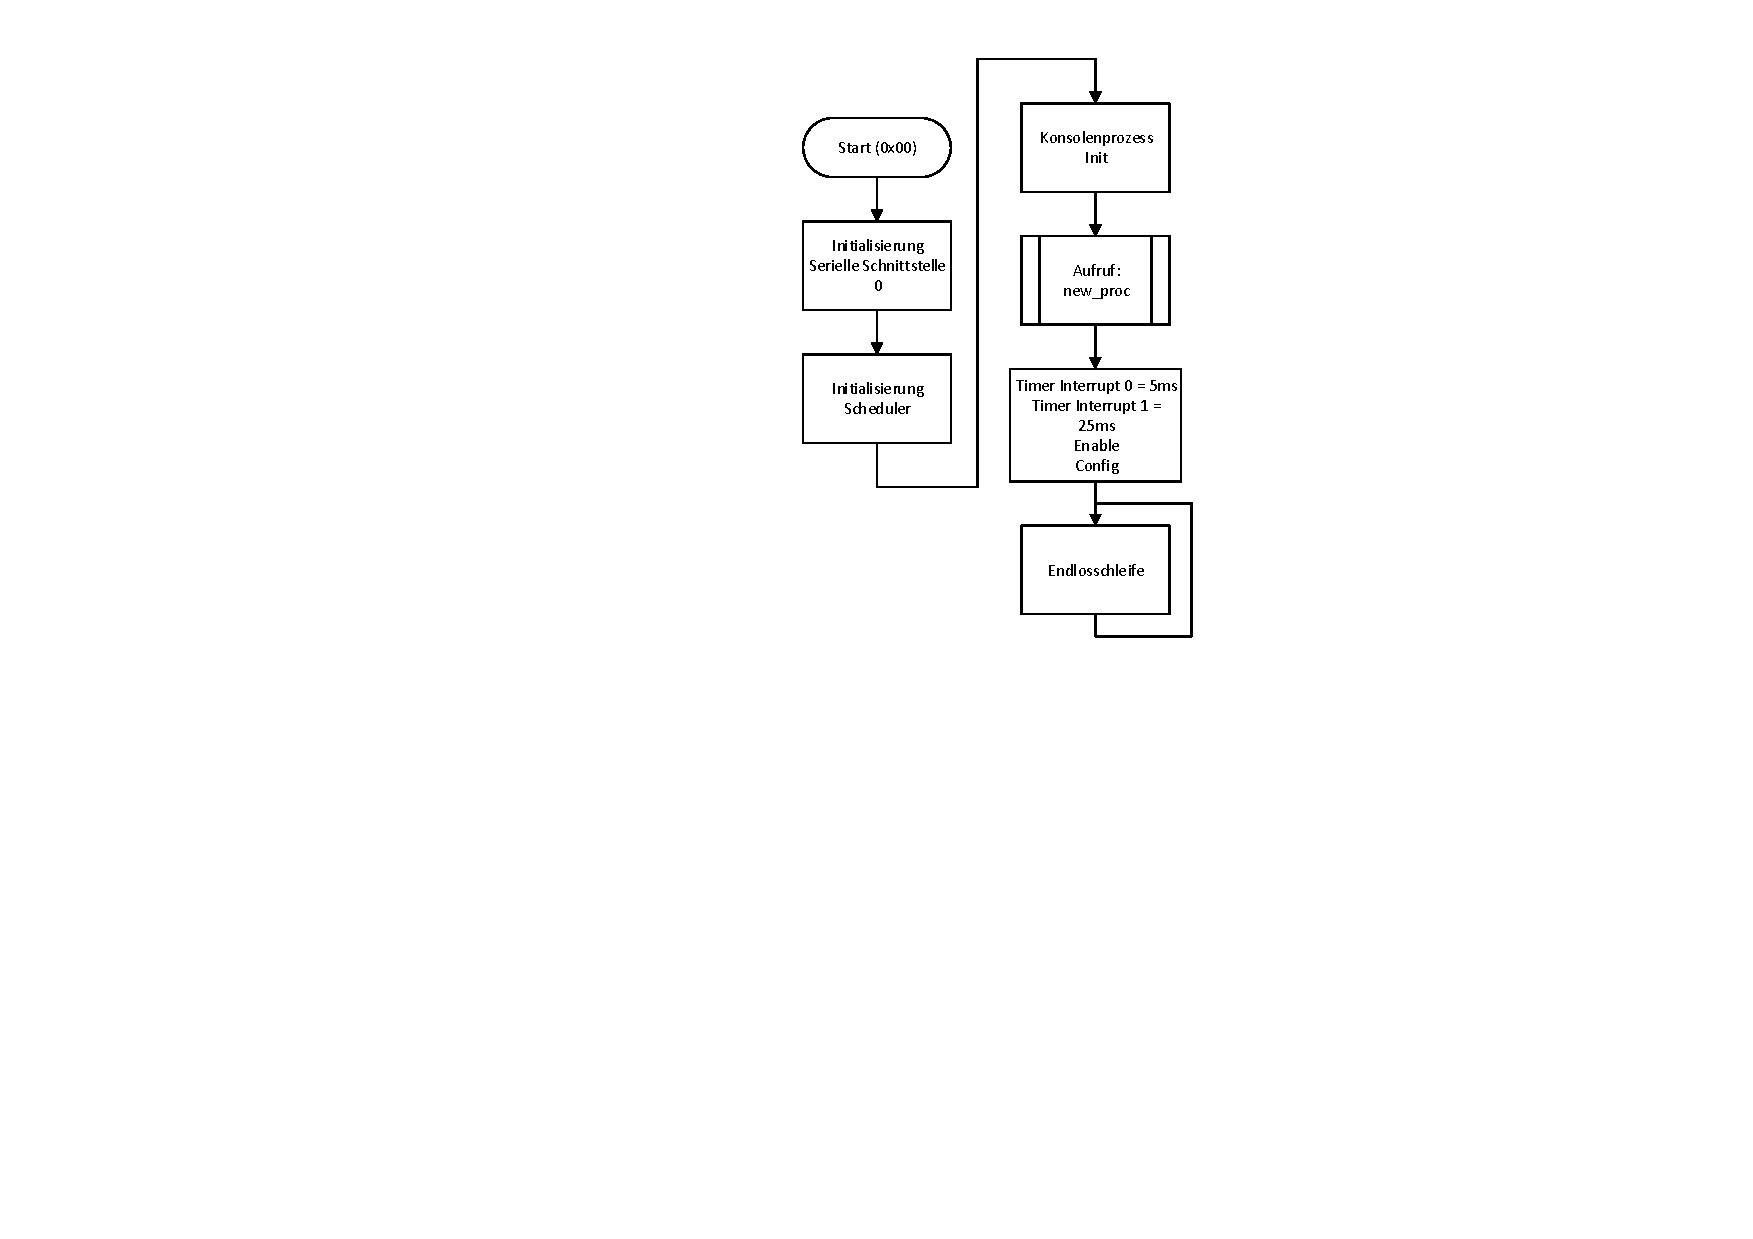
\includegraphics[width=0.5\textwidth]{./images/main}
\caption{Ablaufdiagramm main.a51}
\label{fig:main}
\end{figure}

\subsubsection{Konsolenprozess \texttt{proc\_console.a51}}
In der Abbildung~\ref{fig:console} ist das Ablaufdiagramm vom Hauptmodul dargestellt. Der Konsolenprozess ist eine Endlosschleife. Die genaue Beschreibung der einzelnen Operationen ist aus dem Listing im Anhang zu entnehmen.

Bemerkung: Das Vorbereiten des Prozesses, also das setzen der Parameter ist ein eigenst�ndiger Code-Block. Wegen der �bersicht wird dies als Funktion dargestellt.

\begin{figure}[H]
\centering
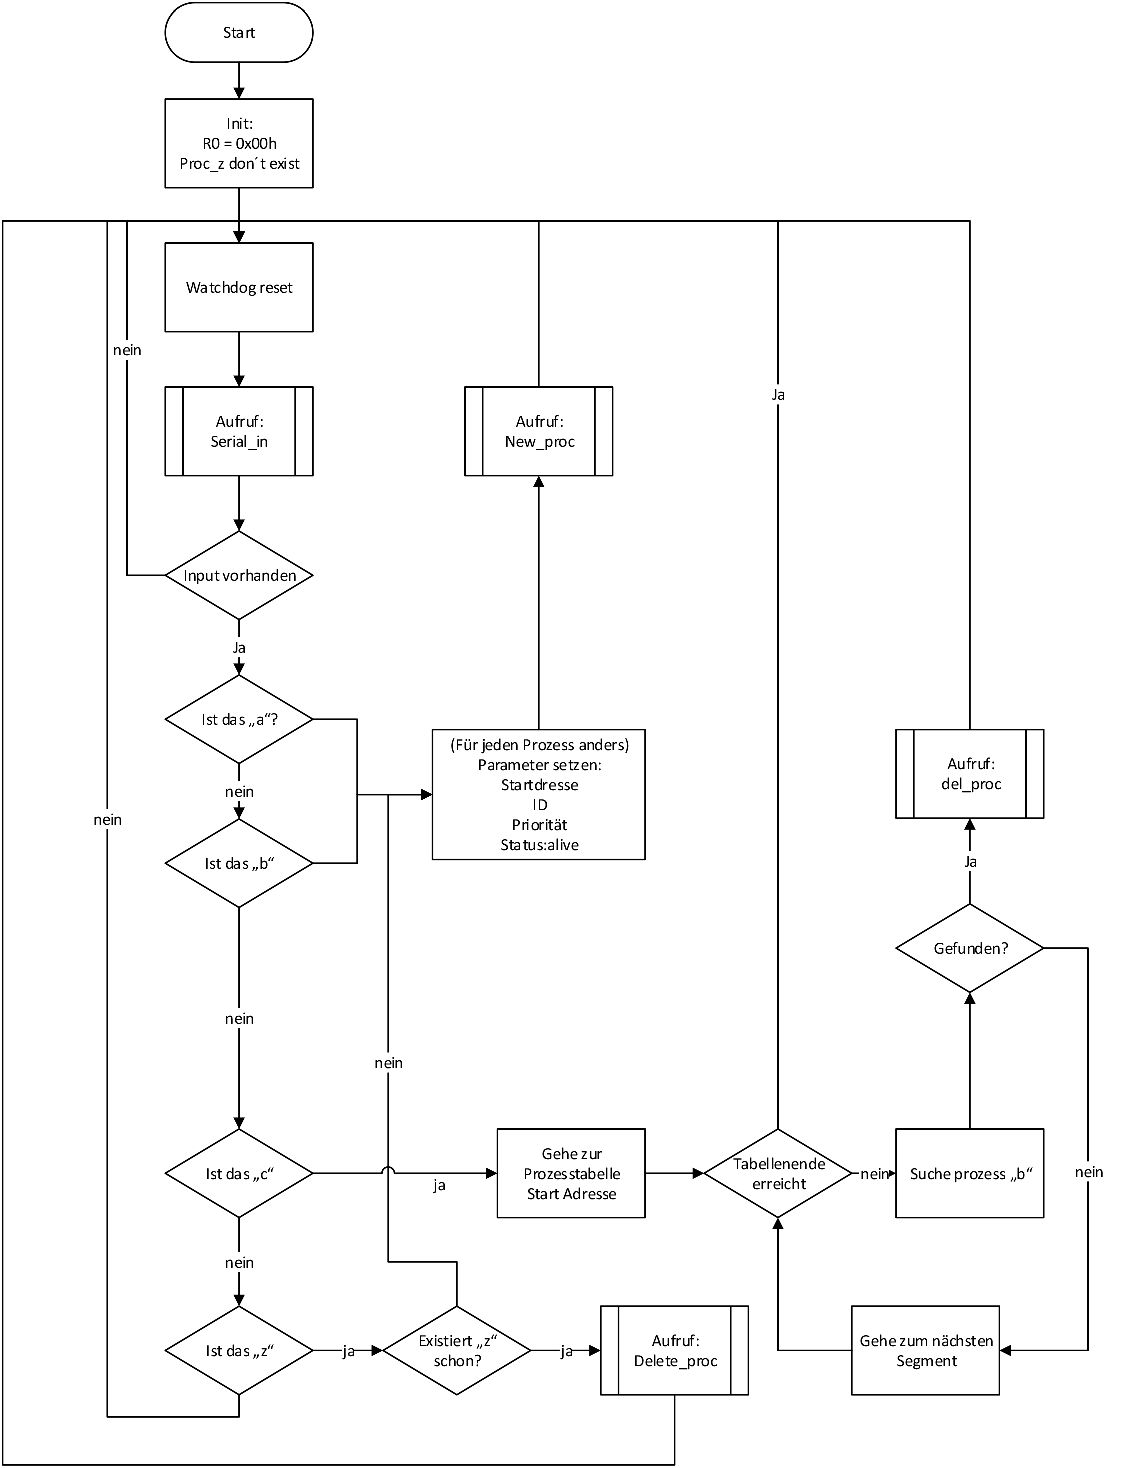
\includegraphics[width=\textwidth]{./images/console}
\caption{Ablaufdiagramm \texttt{proc\_console.a51}}
\label{fig:console}
\end{figure}
\newpage

\subsubsection{Taskverwalter \texttt{scheduler.a51}}

\paragraph{new\_process} In der Abbildung~\ref{fig:newproc} ist das Ablaufdiagramm f�r die Erstellung eines neuen Prozesses dargestellt. Dies ist ein Subprozess des Taskverwalter Moduls. Hierbei werden in die 4 Byte der Prozesstabelle die n�tigen Informationen eingetragen [Startadresse des Prozesses (2 Byte), Bitmaske der Priorit�t und der Prozesstyp ID (1 Byte), Prozess ID (1 Byte) ].


So setzt sich die Bitmaske des 3 Bytes eines Prozess in der Prozesstabelle:

\begin{align*}
B\underbrace{\si{xxxxx}}_{\mathtt{Priorit�t}}\underbrace{\si{xxx}}_{\mathtt{Prozesstyp}}
\end{align*}

Die Prozess ID ist ein HEX-Wert welcher der aktuellen Position des Prozesses in der Tabelle entspricht.

\begin{figure}[H]
\centering
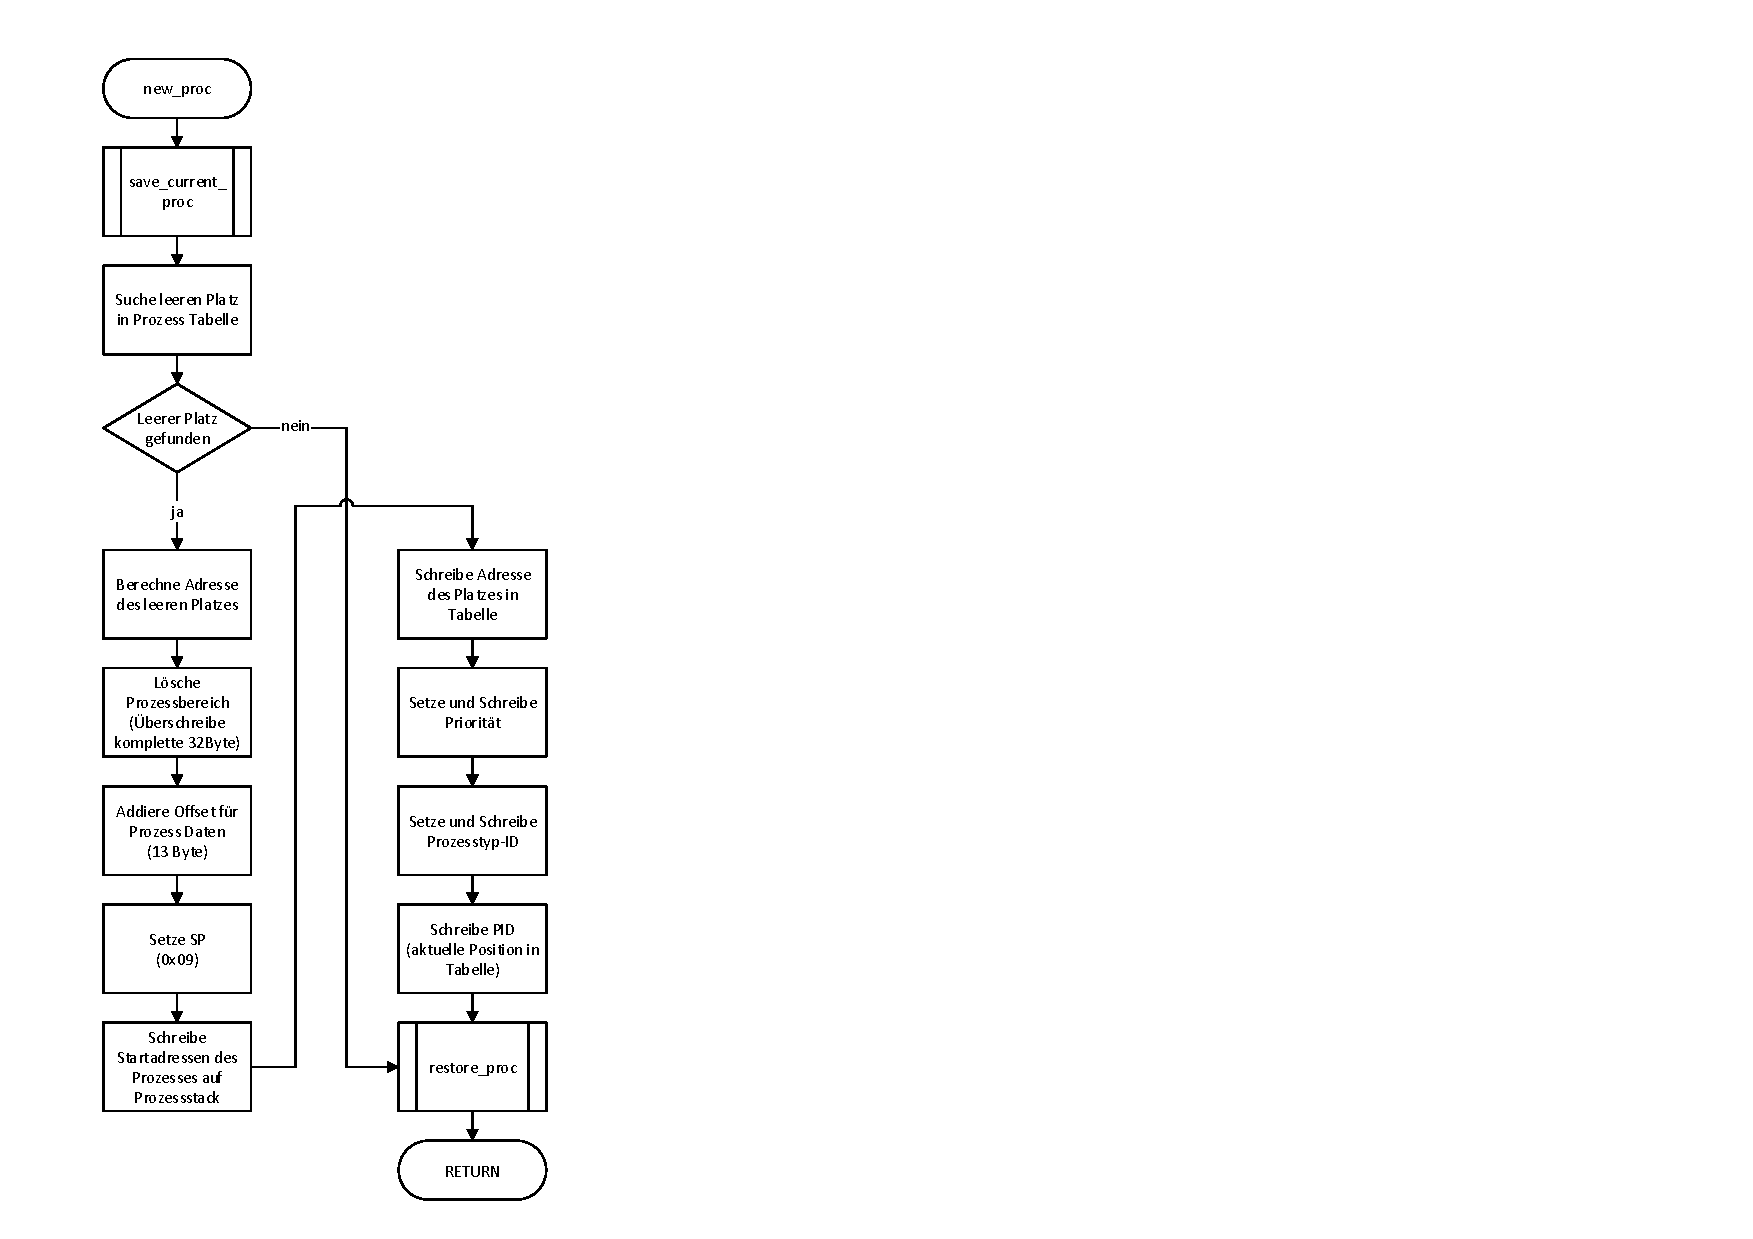
\includegraphics[width=\textwidth]{./images/new_proc}
\caption{Ablaufdiagramm \texttt{newproc}}
\label{fig:newproc}
\end{figure}

\paragraph{delete process}
In der Abbildung~\ref{fig:delproc} ist das Ablaufdiagramm des Subprozesses del\_proc dargestellt. Hierbei werden zun�chst die Daten der aktuellen Routine gerettet. Die Prozesstyp ID wird aus der Bitmaske im 3 Byte der Prozesstabelle extrahiert und mit dem zu l�schenden Typ verglichen. Bei �bereinstimmung wird die Referenz auf den Prozessdatenbereich des zu l�schenden Prozesses entfernt.

Bemerkung: Hier ist es wichtig zu erw�hnen, dadurch dass Prozess b in mehreren Instanzen vorkommen kann und er lediglich durch ein einziges Kommando c gel�scht werden kann, wird der erst beste Prozess vom Typ b auf Kommando gel�scht. Um Prozess gezielt zu entfernen m�sste man das Beenden Kommando anpassen.

\begin{figure}[H]
\centering
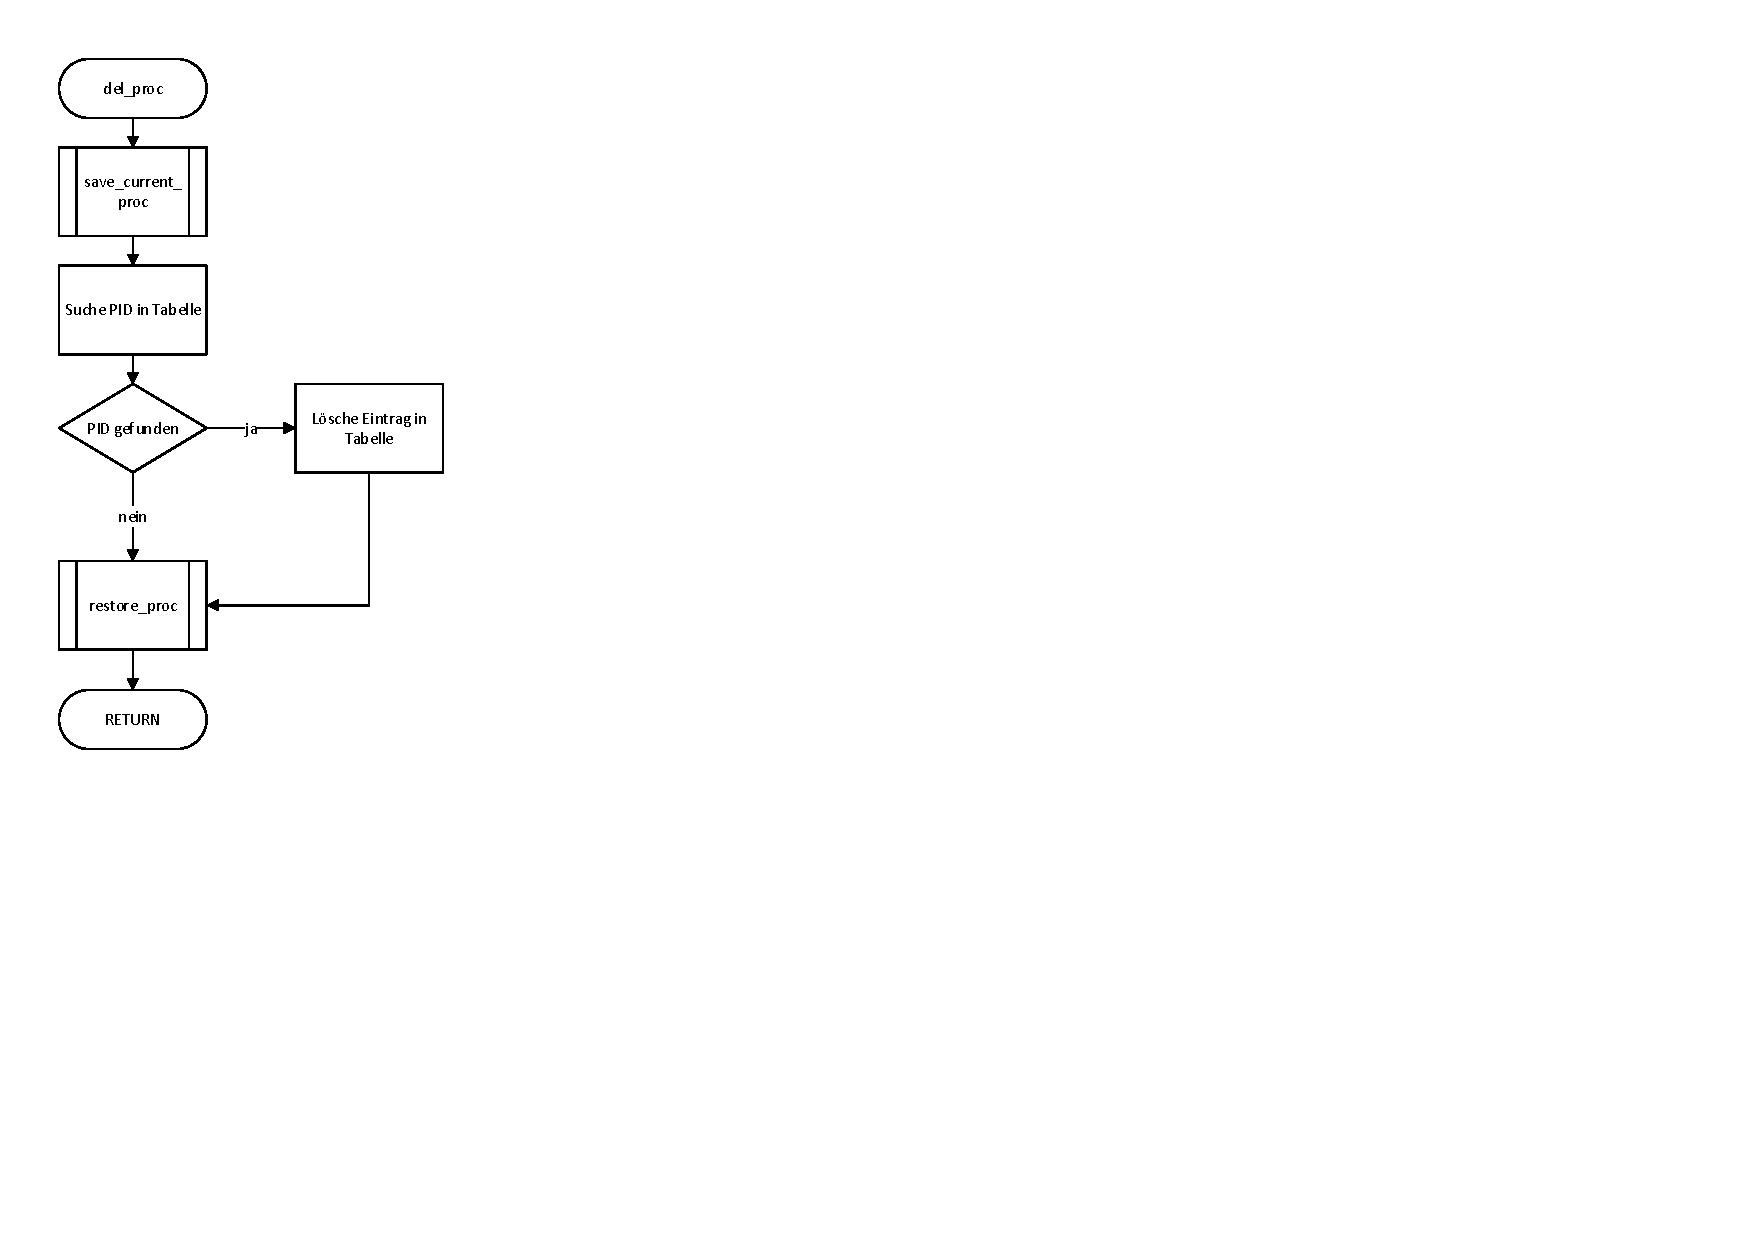
\includegraphics[width=\textwidth]{./images/del_proc}
\caption{Ablaufdiagramm \texttt{delete process}}
\label{fig:delproc}
\end{figure}

\paragraph{change process}

In der Abbildung~\ref{fig:changeproc} ist das Ablaufdiagramm des Subprozesses change process dargestellt. Dieser Subprozess sucht anhand der aktuellen Position des Prozesses den n�chsten in der Prozesstabelle. Da es durchaus leere Eintr�ge geben kann, werden diese �bersprungen. Change process wird nur aufgerufen, wenn ein Prozess seine Zeitscheibe bei der CPU aufgebraucht hat. 

Die Daten des aktuellen Prozesses werden in den externen Prozessdatenbereich ausgelagert und die Daten des neuen Prozesses werden eingeladen. Die Daten werden im Kapitel Speichernutzung erkl�rt.

\begin{figure}[H]
\centering
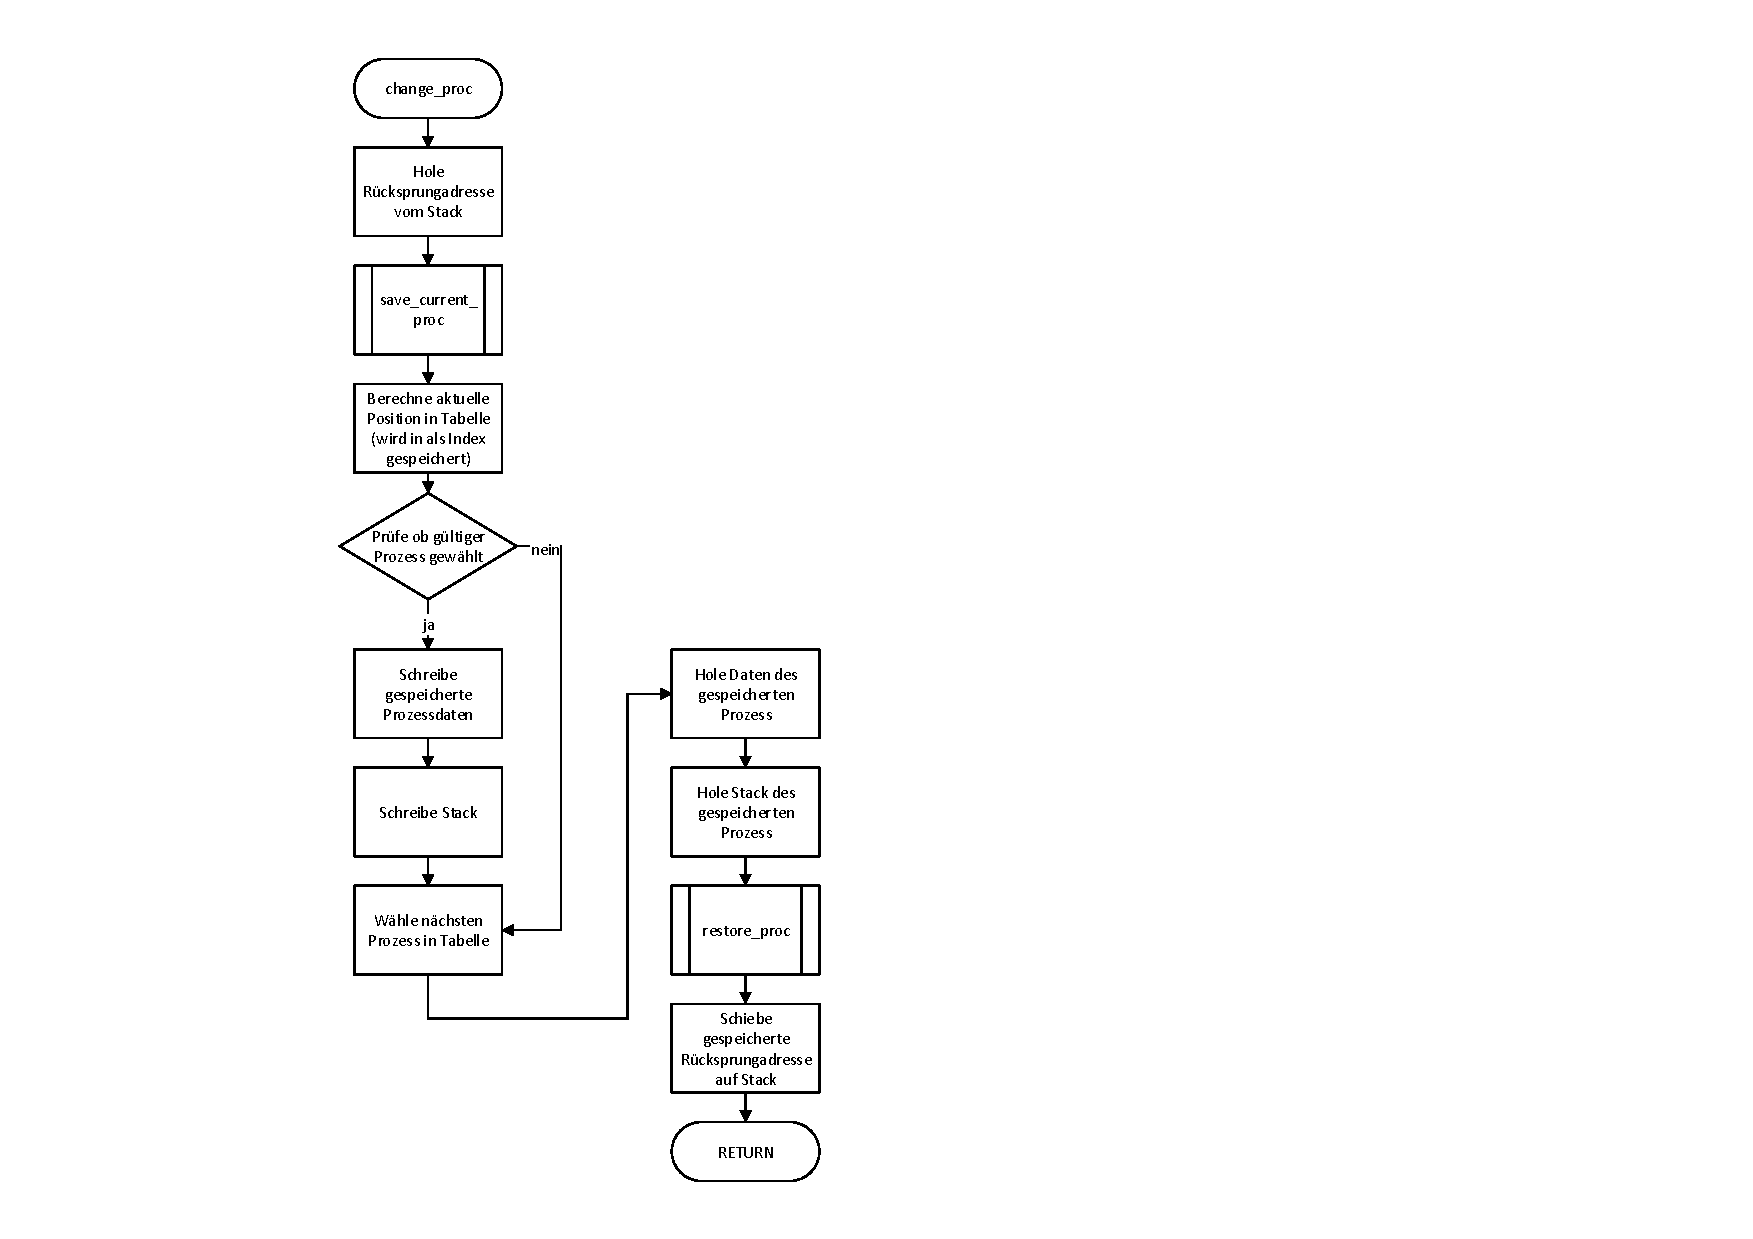
\includegraphics[width=\textwidth]{./images/change_proc}
\caption{Ablaufdiagramm \texttt{change process}}
\label{fig:changeproc}
\end{figure}

\paragraph{save and restore data}
In der Abbildung~\ref{fig:restsavproc} ist die Subroutine zum speichern und retten des Kontexts gezeigt. Die Auflistung der Daten ist dem Kapitel Speichernutzung zu entnehmen.

\begin{figure}[H]
\centering
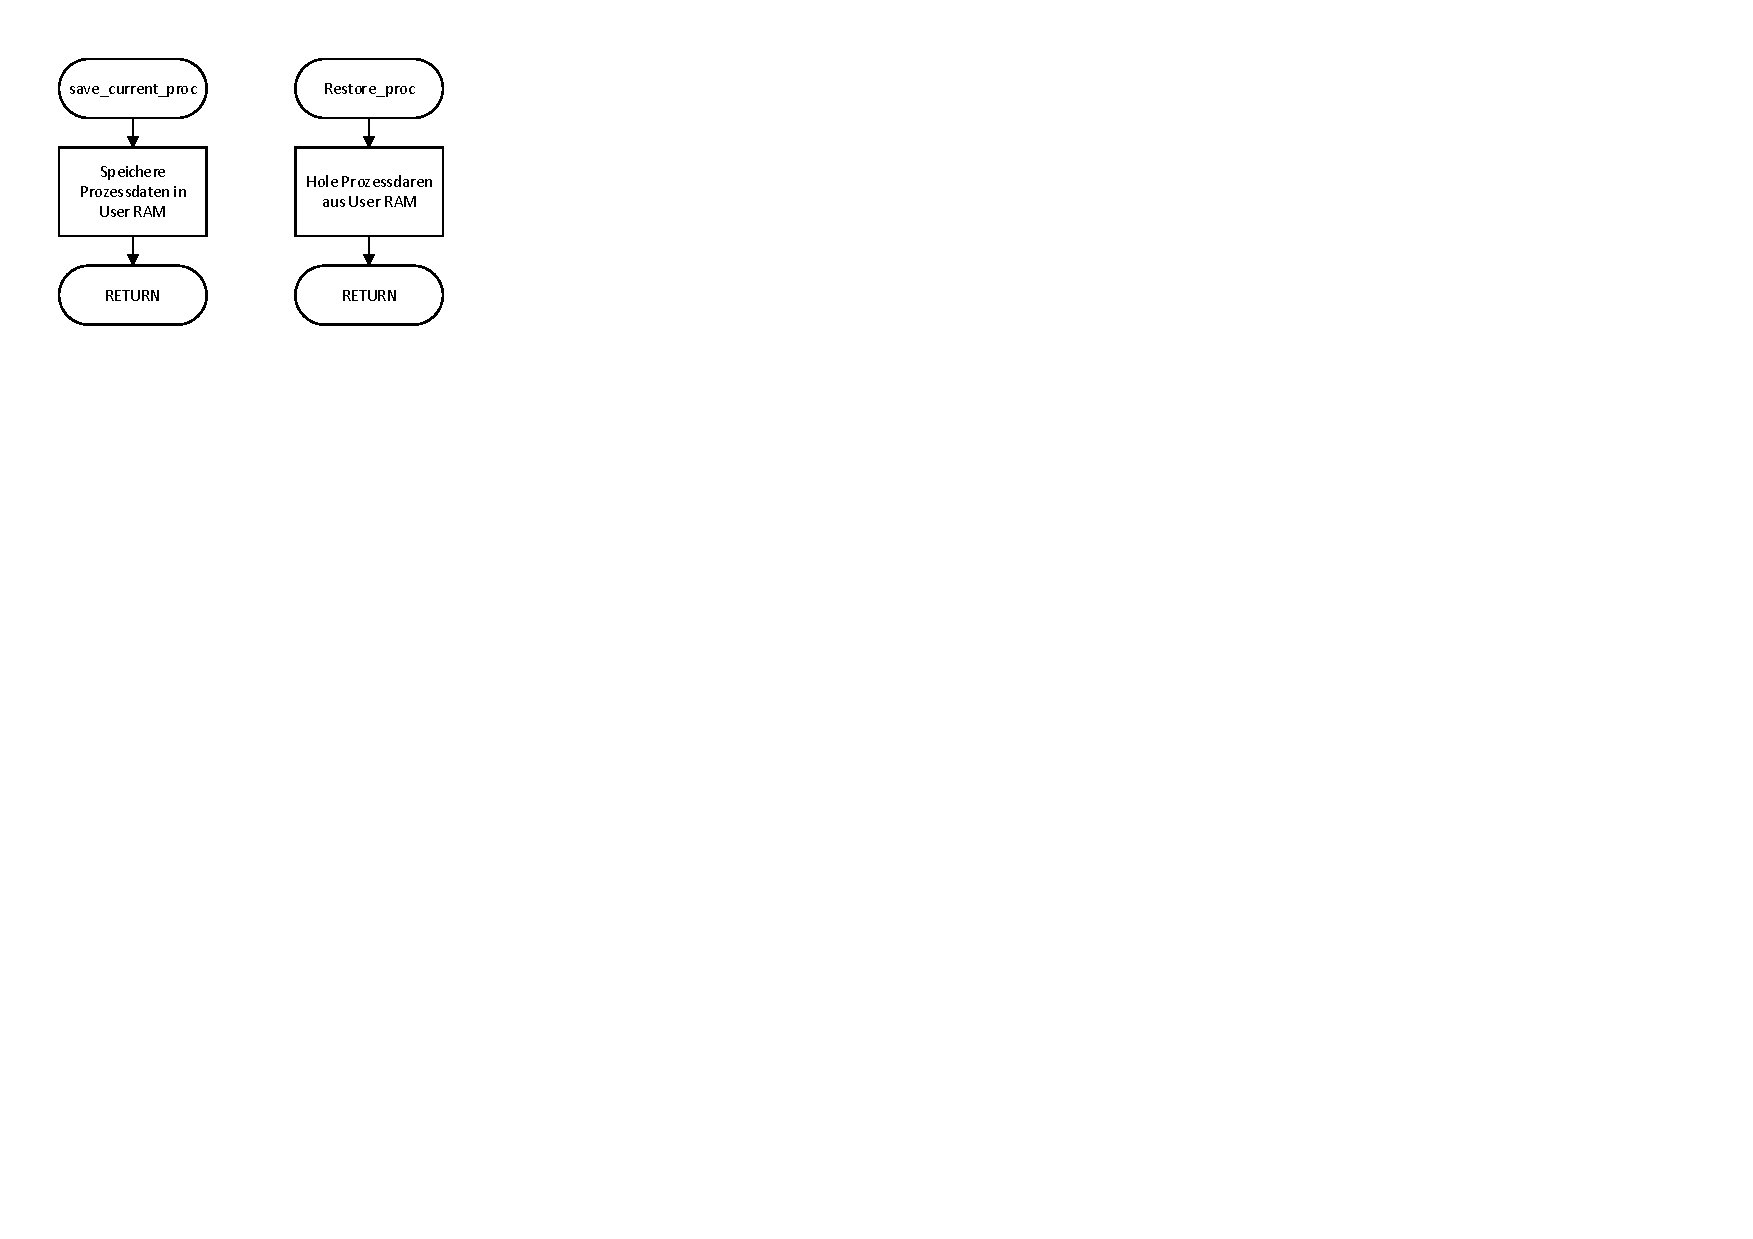
\includegraphics[width=0.6\textwidth]{./images/restore_save_proc}
\caption{Ablaufdiagramm \texttt{restore and save process}}
\label{fig:restsavproc}
\end{figure}

\subsubsection{Serial}
\paragraph{serial init} In der Abbildung~\ref{fig:serialinit} ist die Subroutine serial init dargestellt. Hierbei werden die notwendigen Parameter gesetzt.

	\begin{figure}[H]
		\centering
		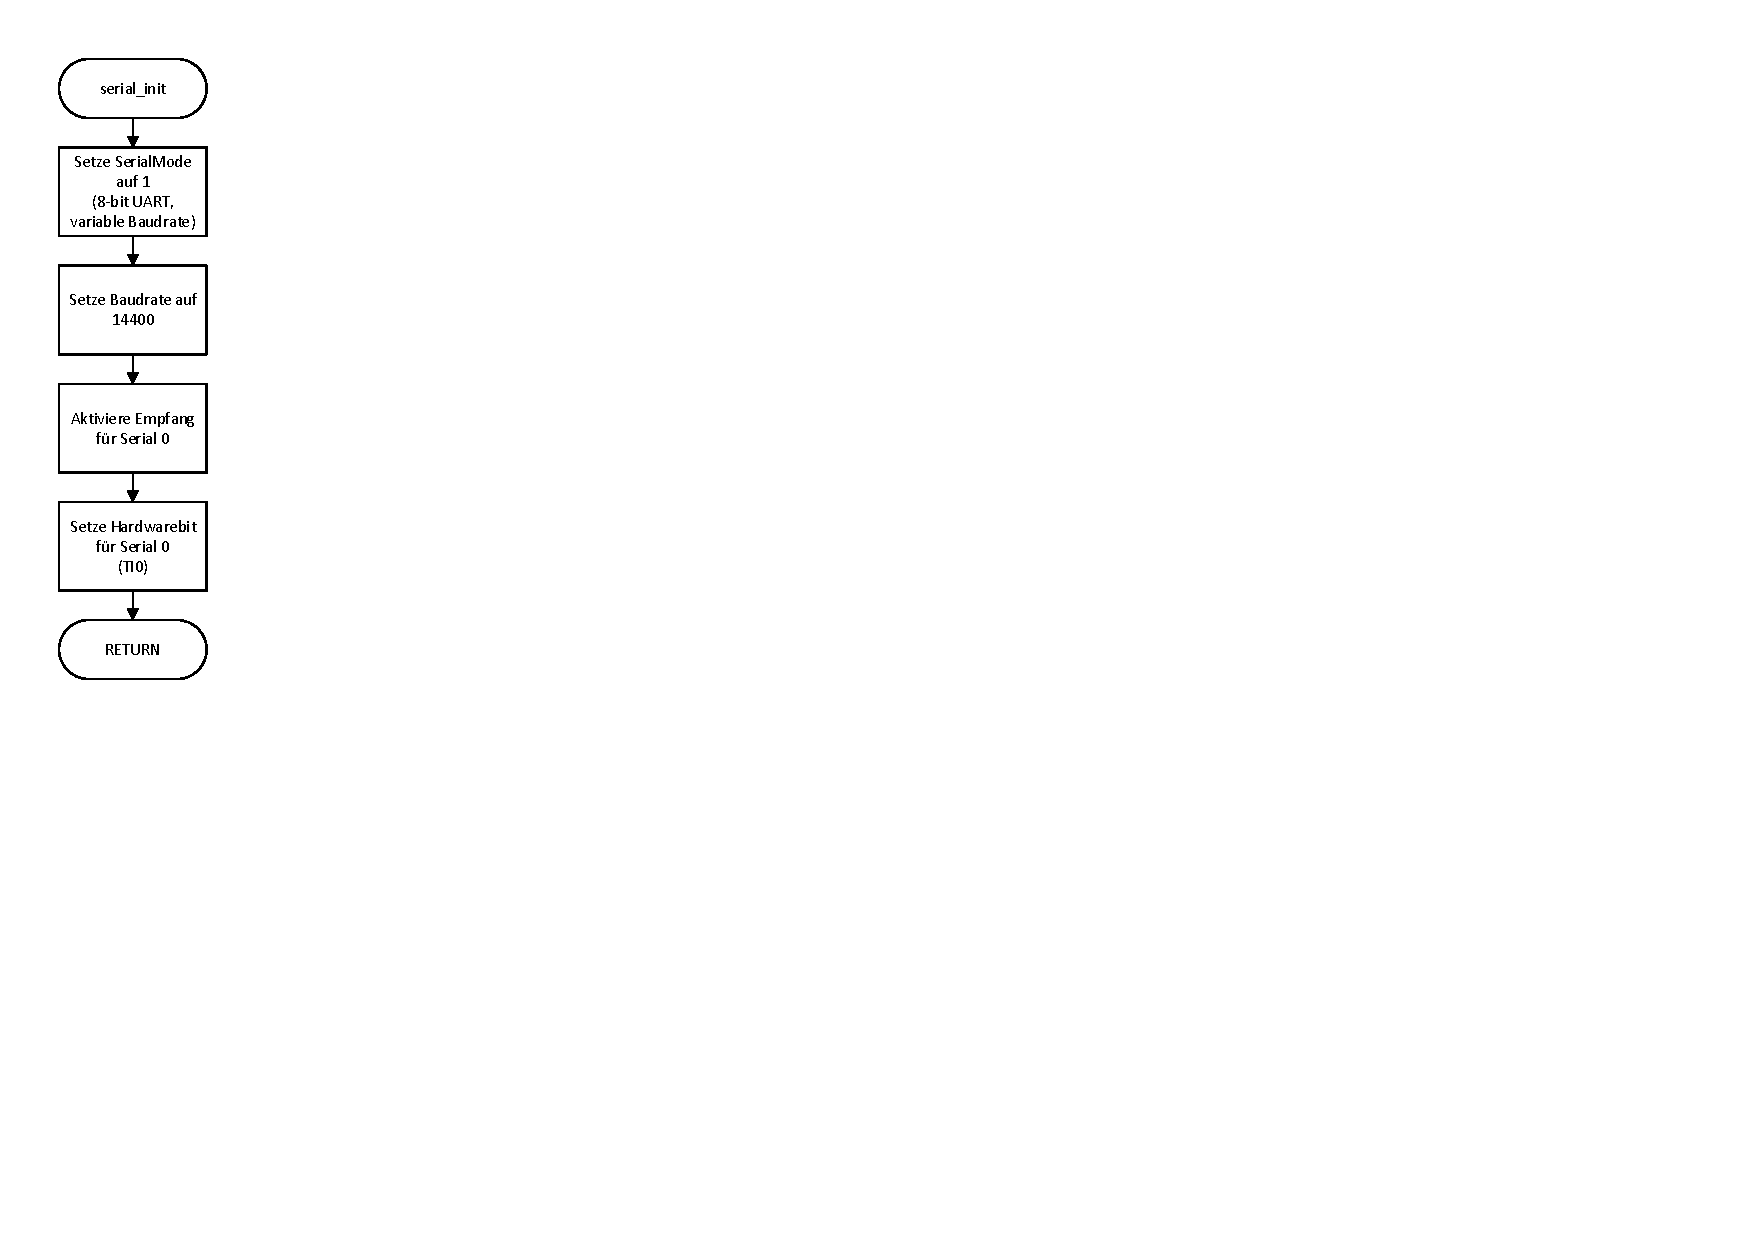
\includegraphics[width=0.3\textwidth]{./images/serial_init}
		\caption{Ablaufdiagramm der Subroutine serial init}
		\label{fig:serialinit}
		\end{figure}


\paragraph{serial in}
In der Abbildung~\ref{fig:serialin} ist die Subroutine serial in dargestellt. Beim ende der Eingabe wird das User Flag F0 gesetzt. Dies ist f�r den Konsolenprozess wichtig. Es k�nnen keine Zeichen verloren gehen, da man nach einem Eingabezeichen bereits die Routine verl�sst.	
	\begin{figure}[H]
		\centering
		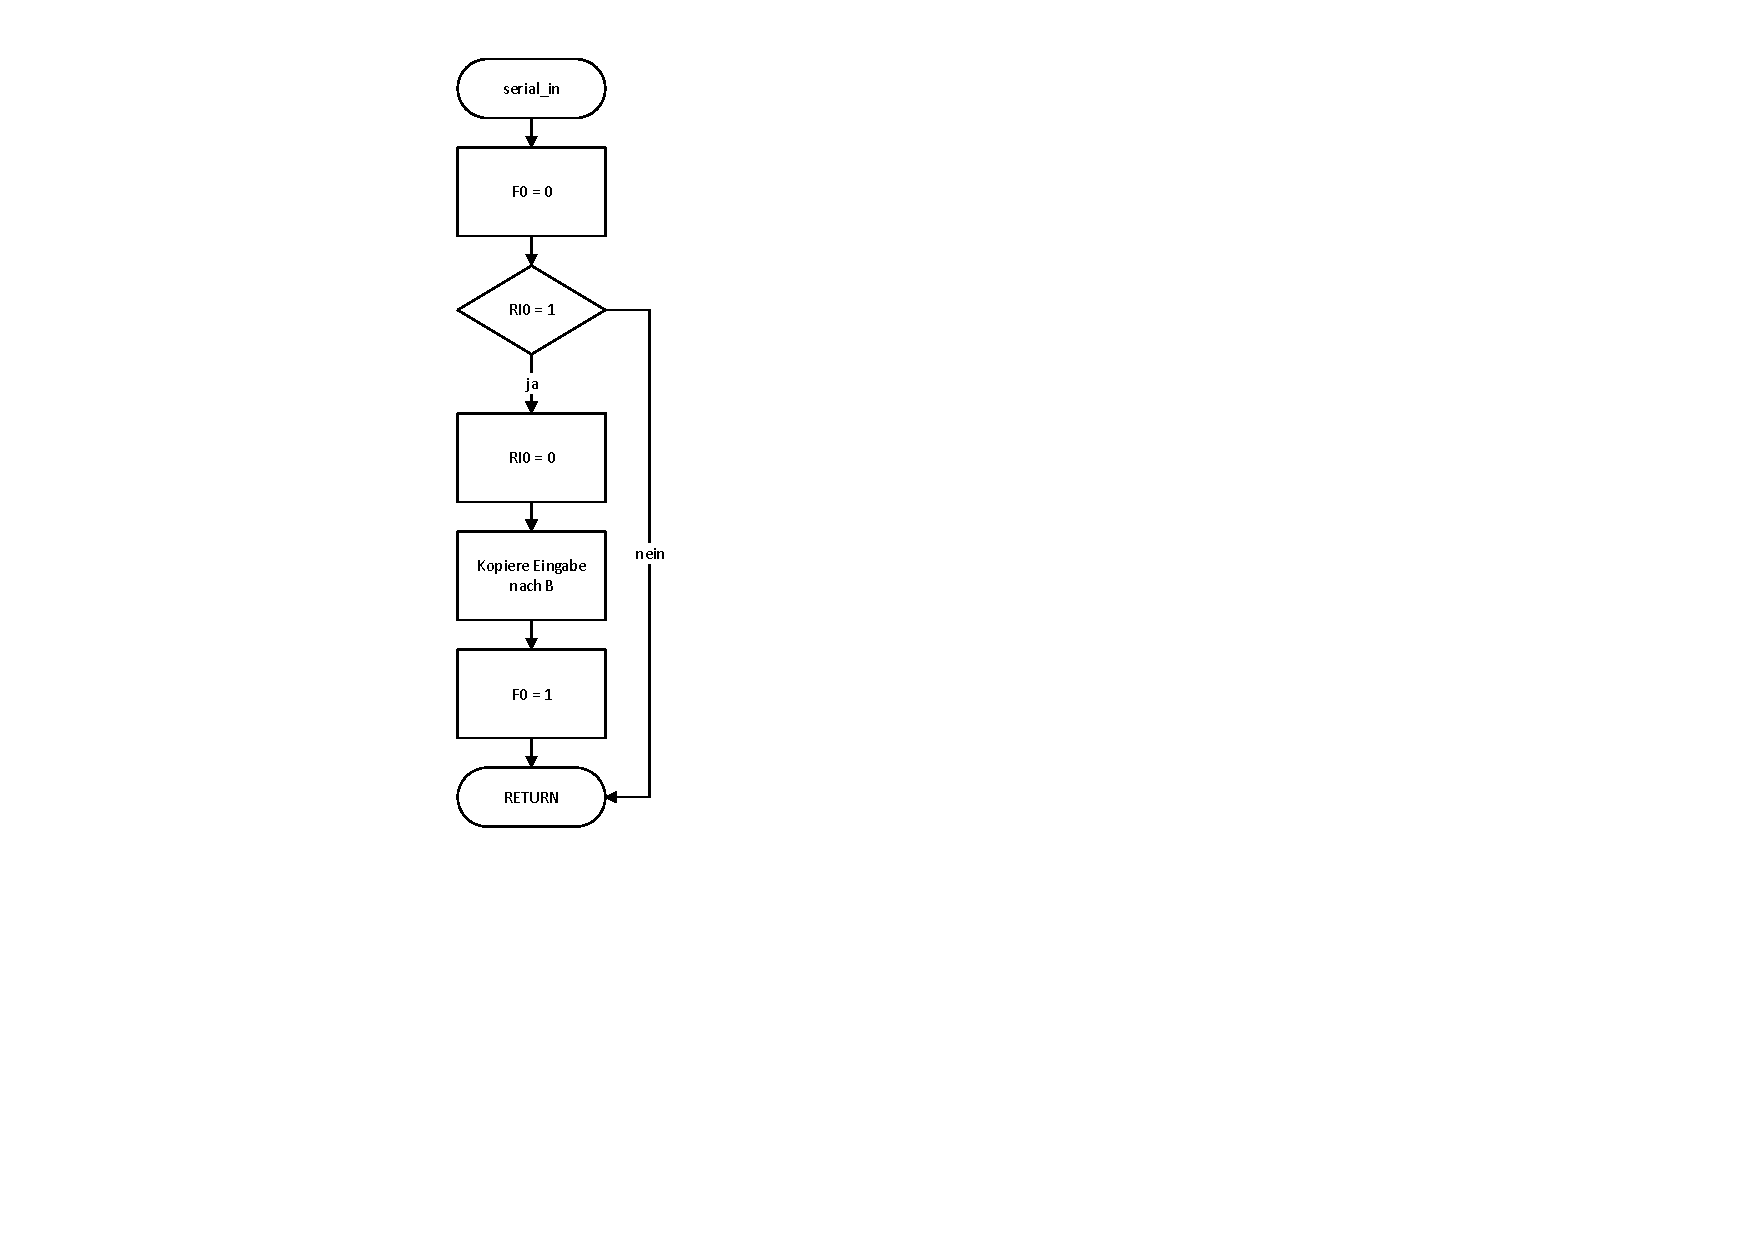
\includegraphics[width=0.3\textwidth]{./images/serial_in}
		\caption{Ablaufdiagramm der Subroutine serial in}
		\label{fig:serialin}
		\end{figure}


\paragraph{serial out}
In der Abbildung~\ref{fig:serialout} ist die Subroutine serial out dargestellt. Es wird Zeichen f�r Zeichen ausgegeben. Es k�nnen auch hier keine Zeichen verloren gehen, da man die Schnittstelle sperrt.

	\begin{figure}[H]
		\centering
		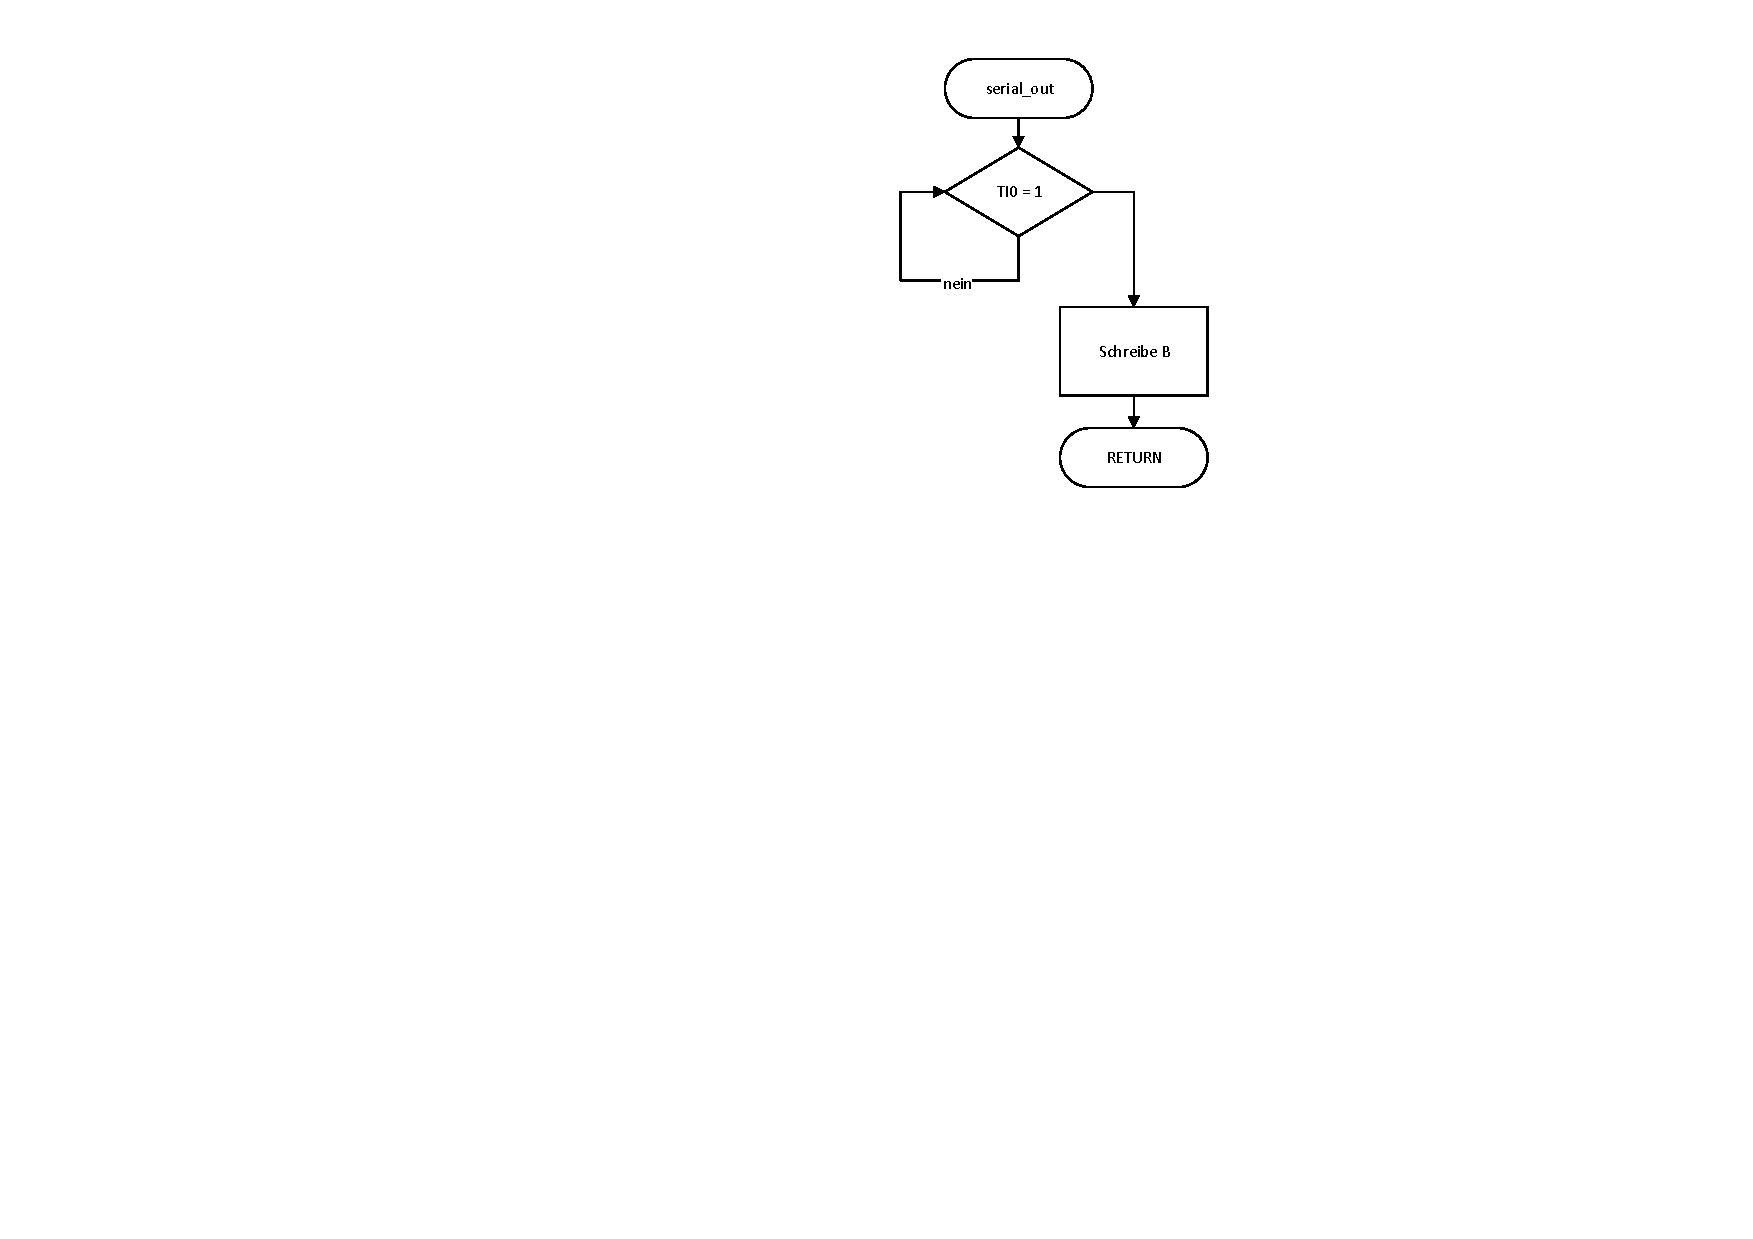
\includegraphics[width=0.3\textwidth]{./images/serial_out}
		\caption{Ablaufdiagramm der Subroutine serial out}
		\label{fig:serialinout}
		\end{figure}


\subsubsection{Prozess a}

In der Abbildung~\ref{fig:proca} ist die Implementierung des Prozess A dargestellt. Prozess A gibt eine Zeichenfolge aus und begibt sich in eine Endlosschleife bis er beendet wird.

		\begin{figure}[H]
		\centering
		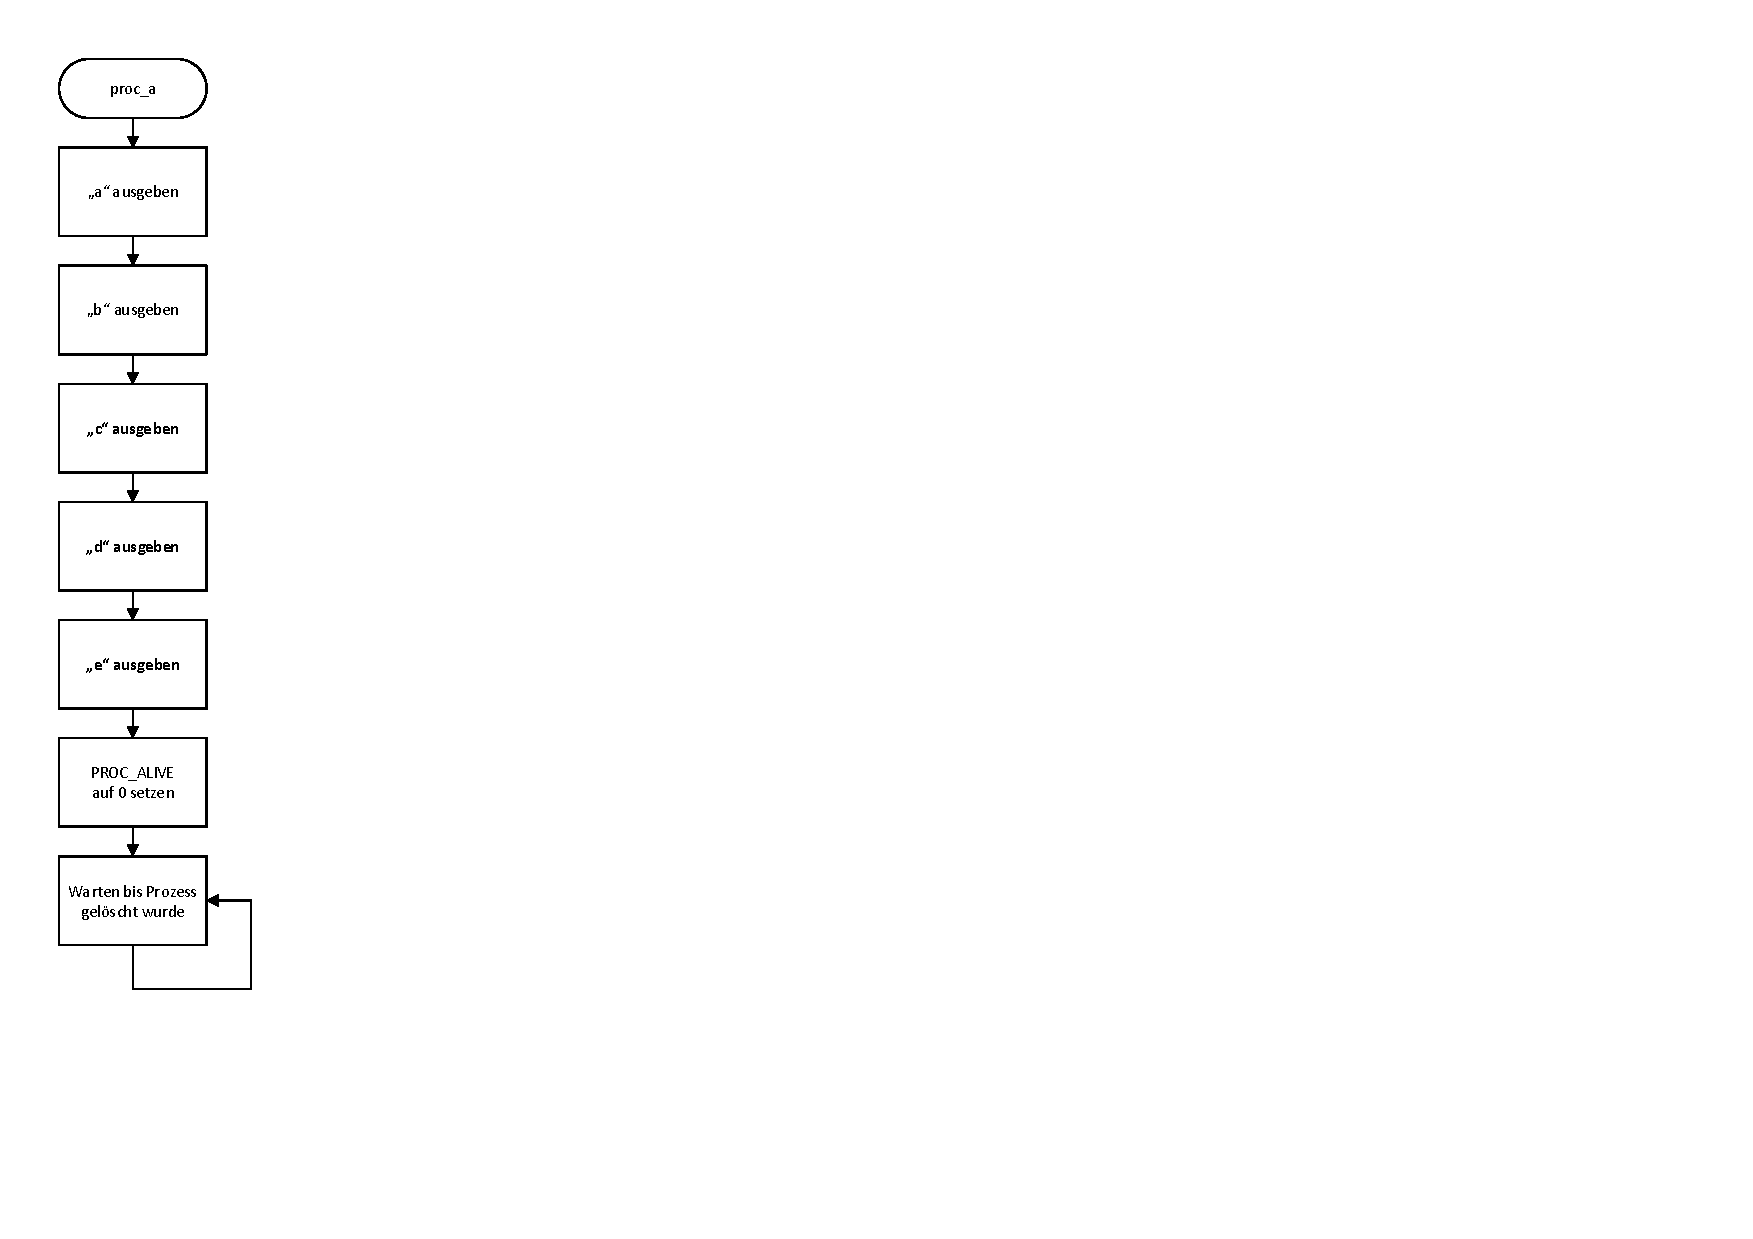
\includegraphics[width=0.3\textwidth]{./images/proc_a}
		\caption{Ablaufdiagramm des Prozess a}
		\label{fig:proca}
		\end{figure}

\subsubsection{Prozess b}
		
		In der Abbildung~\ref{fig:procb} ist die Implementierung des Prozess B dargestellt. Beim Start holt sich der Prozess den aktuellen Wert des Sekundenz�hlers (ganze Sekunden). In einer Schleife wird gepr�ft, ob sich der Systemwert des Z�hlers ver�ndert hat. Hiermit ist eine Sekunde vergangen. Danach wird + Zeichen auf die Konsole ausgegeben. 
		
				\begin{figure}[H]
				\centering
				
\includegraphics[width=0.5\textwidth]{./images/proc_b}
				\caption{Ablaufdiagramm des Prozess b}
				\label{fig:procb}
				\end{figure}

\newpage
